%Figures in this chapter
\newcommand{\Anatomy}{1}
\newcommand{\AnatomyInjection}{\Anatomy A}
\newcommand{\AnatomyThalExample}{\Anatomy B}
\newcommand{\AnatomyThalSummary}{\Anatomy C}
\newcommand{\AnatomyThalamus}{\Anatomy B, C}
\newcommand{\AnatomyACExample}{\Anatomy D}
\newcommand{\AnatomyACSummary}{\Anatomy E}
\newcommand{\AnatomyAC}{\Anatomy D, E}

\newcommand{\Method}{2}
\newcommand{\MethodDiagram}{\Method A}
\newcommand{\MethodDirectCell}{\Method B}
\newcommand{\MethodDirectCellAndNBQXPop}{\Method B, F}
\newcommand{\MethodIndirectNoFollow}{\Method C}
\newcommand{\MethodLongLatency}{\Method C, D}
\newcommand{\MethodIndirectFollows}{\Method D}
\newcommand{\MethodSoundCharPop}{\Method E}

\newcommand{\NoiseLaser}{3}
\newcommand{\NoiseLaserThalDiagram}{\NoiseLaser A}
\newcommand{\NoiseLaserThalExample}{\NoiseLaser B}
\newcommand{\NoiseLaserThalLocations}{\NoiseLaser C}
\newcommand{\NoiseLaserACDiagram}{\NoiseLaser D}
\newcommand{\NoiseLaserACExample}{\NoiseLaser E}
\newcommand{\NoiseLaserACLocations}{\NoiseLaser F}
\newcommand{\NoiseLaserDiagrams}{\NoiseLaser A, D}

\newcommand{\Frequency}{4}
\newcommand{\FrequencyThalExample}{\Frequency A}
\newcommand{\FrequencyACExample}{\Frequency B}
\newcommand{\FrequencyBW}{\Frequency C}
\newcommand{\FrequencyThreshold}{\Frequency D}
\newcommand{\FrequencyLatency}{\Frequency E}
\newcommand{\FrequencyOnsetivity}{\Frequency F}
\newcommand{\FrequencyMonotonicity}{\Frequency G}

\newcommand{\AM}{5}
\newcommand{\AMThalExamples}{\AM A, B}
\newcommand{\AMACExamples}{\AM E, F}
\newcommand{\AMPies}{\AM C}
\newcommand{\AMSync}{\AM D}
\newcommand{\AMRateDiscrim}{\AM G}
\newcommand{\AMPhaseDiscrim}{\AM H}

\chapter{Thalamostriatal and corticostriatal pathways convey complementary information about sound features}

\section{Journal style information}
\noindent Nicholas D Ponvert and Santiago Jaramillo. Reproduced in part from \textit{Journal of Neuroscience}, 2019. Copyright 2019.

\section{Author contributions}
Santaigo Jaramillo provided mentorship for all aspects of the study. Nicholas D Ponvert performed all experiments included in this dissertation. Nicholas D Ponvert and Santiago Jaramillo wrote the sections of the paper pertaining to the results of the experiments included in this dissertation. 

\section{Introduction}
Recent experiments have begun to establish the role of the neural pathway from auditory cortex to the striatum during decision making.
%
Activation of striatal-projecting auditory cortical neurons during a sound discrimination task biases decision making in a frequency-specific way \citep{Znamenskiy2013}, and the synaptic strength between auditory cortical neurons and striatal neurons changes during acquisition of a sound-discrimination task in a way that could support the learned sound-action association \citep{Xiong2015}. 
%
In contrast, the role of the parallel auditory pathway from the thalamus to the striatum is not known.
%
One hypothesis is that this thalamostriatal pathway sends redundant information about sounds, facilitating discrimination of simple, tonal stimuli even after extensive cortical lesions \citep{Gimenez2015, Guo2017}.
%
We hypothesized instead that information about sounds sent by auditory thalamostriatal and corticostriatal neurons is complementary, with specific sound features differentially encoded by these two pathways.

To test this hypothesis, we used an optogenetic approach in awake mice to identify responses from striatal-projecting neurons in auditory thalamus and auditory cortex during extracellular recordings, while presenting sounds of various frequencies and temporal modulations.
%
We found that the two pathways convey information about sound frequency to the striatum with similar fidelity.
%
In contrast, thalamostriatal neurons provide more information about the timing (phase) of amplitude modulated sounds than corticostriatal neurons.
Moreover, the number of evoked spikes in corticostriatal neurons encodes amplitude modulation (AM) rate more accurately than that of thalamostriatal cells. 
%
Downstream circuits capable of linearly decoding spike counts would therefore be better able to discriminate AM rates using corticostriatal inputs compared to thalamostriatal inputs.
%
These findings shed light on the relative contributions of the thalamostriatal and corticostriatal pathways to sound-driven decision making.

\section{Methods}
\subsection{Animals}
%
We used 9 transgenic mice in this study. 
%
Three male and two female transgenic mice expressing Channelrhodopsin-2 in a \textit{Cre} recombinase-dependent manner (LSL-ChR2 mice, JAX number 012569) were used for electrophysiological recordings. 
%
One male LSL-ChR2 mouse was used for NBQX validation of photoidentification methods.
%
Three male mice expressing the fluorescent protein tdTomato in a \textit{Cre} recombinase-dependent manner (Ai14 mice, JAX number 007914) were used in anatomical experiments. 
%
Mice had \textit{ad libitum} access to food and water. Mice used for electrophysiology were between 8 and 14 weeks old at the time of viral injection. 
%
Mice used for anatomy were between 12 and 31 weeks old at the time of viral injection. 
%
All procedures were carried out in accordance with National Institutes of Health Standards and were approved by the University of Oregon Institutional Animal Care and Use Committee.


\subsection{Viral injections}
%
Animals were anesthetized with 2.5\% isoflurane and placed on a stereotaxic surgical apparatus. 
%
The skull was exposed, and a 0.5 mm burr-hole was drilled at the injection coordinates over posterior striatum (A-P: -1.7 mm from bregma, M-L: 3.5 mm right of midline, D-V: -2.75 mm from pia). 
%
A pulled glass pipette (5 $\mu$l, VWR) with a final tip diameter of 15-20 $\mu$m was backfilled with a strain of Canine Adenovirus Type 2 engineered to deliver the gene for \textit{Cre} recombinase (CAV2-Cre, Montpellier Vector Platform) and then lowered into the brain to the injection depth.
%
A 45 nL bolus of CAV2-Cre was then injected manually under air pressure at a rate of 90 nL/min.
%
Two minutes after the injection was complete, the glass pipette was withdrawn 250 $\mu$m.
%
After 1 more minute, the pipette was withdrawn an additional 500 $\mu$m. 
%
After a final 1 minute delay, the pipette was removed and the skin was closed with cyanoacrylate tissue adhesive (VetBond, 3M). 
%
A minimum of 20 days was allowed for expression of the virus before further procedures were carried out. 

\subsection{Electrophysiology and photoidentification of striatal-projecting neurons}
%
In preparation for head-fixed awake electrophysiological recordings, a headbar was attached to the skull of animals under anesthesia.
%
Animals were anesthetized with 2.5\% isoflurane and placed on a stereotaxic surgical apparatus. 
%
The scalp was removed, the headbar was fitted to the skull, and craniotomies were made posterior to the headbar over the coordinates for auditory thalamus (AP: -3.2 mm from bregma, ML: 2.0 mm right of midline) and auditory cortex (AP: -2.8 mm from bregma, ML: 4.4 mm right of midline), ipsilateral to the virus injection.
%
The dura mater was removed. 
%
A plastic well was attached to the skull over each craniotomy and filled with a silicone elastomer (Sylgard 170, Dow-Corning) to protect the brain surface. 
%
Animals were allowed to recover for a minimum of 4 days before beginning electrophysiology experiments.

On each recording session, animals were head-fixed and allowed to run on a wheel inside a single-walled sound-isolation box (IAC-Acoustics). 
%
The silicone plug was removed from the well, and electrodes were inserted through the well into the brain. 
%
All recordings were performed with 4-shank, 32-channel silicon probes with electrodes arrayed in tetrodes (A4x2-tet-5mm-150-200-121, NeuroNexus). 
%
Data were collected using an RHD2000 acquisition system (Intan Technologies) and the OpenEphys software (\url{http://www.open-ephys.org/}).
%
Shanks were marked with a fluorescent dye (DiI: Cat \#V22885, or DiD: Cat \#V22887, Thermo-Fisher Scientific) before penetration to facilitate post-mortem imaging of electrode tracts. 
%
Silicon probes were fitted with a 50 $\mu$m diameter optical fiber (Polymicro Technologies) placed between the two middle shanks and terminating 450 $\mu$m from the tip of the probe (200 $\mu$m above the tetrode farthest from the tip). 
%
This optical fiber was used to deliver 445 nm laser light (1.5 mW at the fiber tip).

To find striatal-projecting neurons, we presented 100 ms pulses of light and 100 ms bursts of 60 dB SPL white noise. 
%
We continued recording only if we found both light-evoked and sound-evoked responses. 
%
We next presented trains of 10 ms light pulses at 5 Hz to distinguish between neurons expressing ChR2 and those indirectly activated via synaptic input from ChR2-positive neurons \citep{Lima2009}, see ``Automatic selection of ChR2-tagged neurons.''
%
Last, we presented the ensemble of auditory stimuli to determine frequency tuning and responses to amplitude modulation. 
%
After the recording was complete, the silicon probe was removed and the well was re-filled with silicone elastomer. 
%
Multiple recordings were performed for each animal (one recording per day). 
%
After the last recording session, animals were sacrificed and their brains were extracted.

\subsection{Validation of photoidentification methods}
To validate approaches for discriminating between neurons directly activated by ChR2 and neurons that were indirectly activated by synaptic input, we evaluated the effects of blocking synaptic transmission using the AMPA glutamate receptor antagonist NBQX (\#N183, Sigma-Aldrich). 
%
We performed electrophysiological recordings from the auditory cortex of an LSL-ChR2 mouse that had been injected with CAV2-Cre in the posterior striatum.
%
After the electrodes and optical fiber were inserted in the brain, we inserted a pulled glass pipette (identical to those used for virus injection) loaded with NBQX (10 mM, dissolved in sterile saline) so that the tip was located near the electrodes.
%
We recorded responses of neurons to 100 ms bursts of white noise, 100 ms laser pulses, and trains of 10 ms laser pulses presented at 5 Hz. 
%
We then injected 180-360 nL of NBQX under air pressure at a rate of 90 nL/min.
%
After the injection was complete, we presented white noise stimuli to evaluate sound-evoked responses.
%
When sound evoked responses were completely suppressed, we recorded post-injection responses to the laser stimuli.


\subsection{Auditory stimuli}
Auditory stimuli were presented in open-field configuration from a speaker (MF1, Tucker-Davis Technologies) contralateral to the side of recording. 
%
Speakers were calibrated using an ultrasonic microphone (ANL-940-1, Med Associates, Inc.) to obtain the desired sound intensity level for frequencies between 1 kHz and 40 kHz. 
%
Stimuli were created using the \textit{taskontrol} platform (\url{www.github.com/sjara/taskontrol}) developed in our laboratory using the Python programming language (\url{www.python.org}). 
%
The ensemble of auditory stimuli was composed of white noise bursts (100 ms duration, 60 dB SPL, 100 repetitions), pure tone pips at 16 frequencies logarithmically-spaced between 2 and 40 kHz (100 ms duration, 15-70 dB SPL in 5 dB steps, 10 repetitions per condition), and sinusoidally amplitude modulated white noise at 11 modulation rates logarithmically-spaced between 4 and 128 Hz (100\% modulation depth, 500 ms duration, 60 dB SPL max, 50 repetitions per condition).
%
All stimuli had a 2 ms ramp up and ramp down. 
%
Interstimulus intervals were randomized (700-900 ms) to prevent the mouse from being able to predict the onset of the stimulus. 

\subsection{Histology}
Animals were deeply anesthetized with euthasol and then perfused through the heart with 4\% paraformaldehyde.
%
Brains were extracted and left in 4\% paraformaldehyde for at least 24 hours before slicing. 
%
Brains were sliced under phosphate-buffered saline on a vibratome. 
%
For anatomical experiments, slice thickness was 75 $\mu$m. 
%
For verification of electrode tracts and viral injection after electrophysiology experiments, slice thickness was 50 $\mu$m.
%
Brain slices were imaged with a fluorescent microscope (Axio Imager 2, Carl Zeiss) with a 5x objective (NA 0.16).
%
Animals were considered for analysis only if the viral injection was well-localized to the posterior striatum. Labeled neurons along the injection tract were observed in one of the anatomy animals, but results for this animal were not qualitatively different from other animals.

\subsection{Experimental Design and Statistical Analysis}
All statistical comparisons were performed using two-sided non-parametric statistical tests with no assumption of normality.
%
During identification of fluorescent neurons in histology slices, the experimenter was presented only with the fluorescence channel so they would be blind to the surrounding anatomy of the area. 
%
All ChR2-tagged neurons were selected by an automated method without experimenter input.
Full details regarding the statistical analysis for each experiment are described in the sections below. 


\subsection{Cell counting}
%
For counting labeled neurons in auditory thalamus, we analyzed each brain slice that contained any part of the medial geniculate nucleus. 
%
This set of slices was divided into 3 interleaved sets of sections, which were analyzed independently to provide an estimate of the variability for each animal.
%
For auditory cortex, we counted labeled neurons in 4 slices in the middle of primary auditory cortex.
%
We first identified coordinates of labeled neurons.
%
We then manually registered each histology slice to the corresponding coronal section in the Allen Mouse Common Coordinate Framework (Common Coordinate Framework v.3, © 2015 Allen Institute for Brain Science, Allen Brain Atlas API, available from \url{http://brain-map.org/api/index.html}). 
%
We used this registration to determine the brain area of each labeled neuron.


\subsection{Spike sorting}
Spiking activity was detected by applying a low threshold (25-30 $\mu$V) to band-pass (300 to 3000 Hz) filtered continuous data.
%
Spiking activity of single units was isolated offline using the automated expectation maximization clustering algorithm Klustakwik \citep{Kadir2014}. 
%
Isolated clusters were only included in the analysis if less than 2\% of inter-spike intervals were shorter than 2 ms. 
%
Clusters with 2-4\% of inter-spike intervals shorter than 2 ms were automatically refined by iteratively removing the spike with the largest Mahalanobis distance to the cluster centroid in feature space until the cluster had less than 2\% of inter-spike intervals shorter than 2 ms.
%
We confirmed by visual inspection that the waveform-amplitude distributions of the resulting clusters were Gaussian.
%
%We also calculated a spike quality index, defined as the ratio between the magnitude of the sodium peak and the average variance for the largest channel.
We also calculated a spike quality index, defined as the ratio between the peak amplitude of the waveform and the average variance, calculated using the channel with the largest amplitude.
%
We included cells with spike quality indices greater than 2. 


\subsection{Automatic selection of ChR2-tagged neurons}
%
We used an automatic method to select neurons that were directly tagged with ChR2. 
%
We first required neurons to have statistically significant responses above baseline (p$<$0.05) within the first 10 ms of a 100 ms pulse of 445 nm laser light.
%
We then required that neurons have a statistically significant response above baseline (p$<$0.05) to the first 10 ms pulse of the 5 Hz train of pulses, and to 3 out of the 4 subsequent pulses. 
%
Last, we required neurons to reach 1/2 of their maximum laser pulse-evoked firing rate within 10 ms of the pulse onset.
%
Using stricter values for this criterion (\emph{e.g.}, 6 ms) resulted in exclusion of additional cells, but did not qualitatively affect our results.

\subsection{Estimation of frequency tuning}
%
We used an automated method to determine the characteristic frequency (CF), threshold, and frequency tuning bandwidth of each cell.
%
We first determined the frequency response area (FRA) defined as the set of frequency-intensity pairs for which the cell’s response was greater than a response threshold, defined as the baseline firing rate plus 20\% of the difference between baseline and the cell’s maximum firing rate under any condition \citep{Sutter1991, Schumacher2011}.
%
Using more stringent criteria (30\% or 40\% of the difference between baseline and maximum firing) resulted in exclusion of some cells, but did not qualitatively affect our results.
%
The neuron’s CF was defined as the frequency with the lowest sound intensity inside the FRA where 85\% of the intensities above were also within the FRA.

For neurons with sound intensity thresholds at 60 dB SPL or below, we fit a Gaussian curve to the individual trial stimulus-evoked spike counts across frequencies at 10 dB above the sound intensity threshold. 
%
We then found the upper intersection ($f_{upper}$) and lower intersection ($f_{lower}$) of this curve with the same response threshold value that we used to define the FRA. 
%
We defined the bandwidth at 10 dB above the neuron's sound intensity threshold (BW10) to be: ($f_{upper} - f_{lower})/CF$.
%
Our comparisons of tuning width included only neurons for which the Gaussian function fit the data with an R-squared value above 0.04 (to remove cells with very noisy responses) and had a midpoint below 32 kHz (to prevent estimation of upper tuning flanks outside the range of the frequencies tested). 

\subsection{Comparison of onset \emph{vs.}\ sustained response to sound}
We calculated the firing rate in response to presentations of each cell's characteristic frequency during two time bins after sound onset.
%
Only trials in which the the CF was presented at 50-70 dB SPL were used in this analysis.
%
The onset period was defined as the time range from the response latency of the cell to latency + 50 ms.
%
The sustained time range was defined as latency + 50 ms to latency + 100 ms.
%
Defining time ranges relative to the latency of each individual neuron was necessary to prevent underestimation of the onset component for neurons with longer latencies.
%
We then calculated an index for the relationship between the onset and sustained portions of the response, defined as: (onset - sustained ) / (onset + sustained). 
%
We also performed this comparison using responses to AM sounds.
%
In this case, the sustained period was defined as latency + 50 ms to latency + 500 ms.
%For this comparison, the onset period was defined as from the latency of the cell to latency + 50 ms.
%
%The sustained time range was defined as latency + 50 ms to latency + 500 ms.

\subsection{Estimation of monotonicity of response with respect to sound level}

We estimated the monotonicity of each neuron's response to presentations of its characteristic frequency at different intensities. We first calculated the firing rate during the sound. We then calculated an index of monotonicity used in previous studies \citep{DelaRocha2008, Watkins2011}, defined as the ratio between the firing rate at the maximum intensity and the maximum firing rate at any intensity.

\subsection{Estimation of AM synchronization}
We computed the vector strength (a measure of the synchronization between the spike times for a neuron and the period of the sinusoidal amplitude modulation function) for the responses to each AM rate.
%
We discarded any spikes from the first 100 ms after stimulus presentation for this analysis (to avoid overestimating synchronization due to strong onset responses).
%
We then performed Rayleigh’s test to determine the AM rates for which a neuron displayed statistically significant (p$<$0.05) synchronization of its firing with respect to the phase of the amplitude modulation. 
%
Since this test was performed for each of the 11 AM rates presented, we performed a Bonferroni correction for multiple comparisons ($\alpha$ = 0.05/11 = 0.0045).
%
For each neuron, we estimated the highest AM rate where the neuron’s firing was significantly synchronized to the modulation period. 

\subsection{Stimulus discrimination based on neural activity}
For linear discrimination of AM rates given the activity of each neuron, we first calculated the number of spikes fired over the duration of the stimulus on each trial.
%
We determined the AM rate that elicited the most spikes on average (preferred) and the AM rate that elicited the least spikes on average (least-preferred).
%
We then found the spike-count threshold that best discriminated between preferred and least-preferred stimuli using exhaustive search.  
%
Because preferred and least-preferred stimuli were chosen from the data, this method has a discrimination chance level slightly above that of a balanced classification task: 60\% in our case (estimated as the average of shuffling AM rates, 1000 repetitions).

To calculate how accurately a linear discriminator could tell apart different times during the cycle of the AM stimulus, we first aligned all spikes to the period of the sinusoidal envelope.
%
For each AM rate, we divided the period of the stimulus up into 4 bins and found the bin with the highest average spike count (the preferred phase) and the lowest average spike count (the least-preferred phase).
%
Similar to above, we found the spike-count threshold that best discriminated between preferred and least-preferred stimuli using exhaustive search. 
%
Chance level was estimated to be 55\% by shuffling period bin numbers, 1000 repetitions. 


\subsection{Mutual information}
%
We computed the mutual information (MI) between the average firing rate over the entire 500 ms AM stimulus and the AM rate on each trial. 
%
To account for potential overestimation of mutual information due to having only a limited number of trials for each condition, we repeatedly (500 times) calculated the mutual information between the average firing rate and a shuffled version of the AM rates. 
%
We subtracted this estimate of the bias from the original estimate of MI to obtain a bias-corrected estimate of MI.


\section{Results}

\subsection{Auditory cortex and auditory thalamus send sound information to the posterior striatum}

We first determined which regions of auditory thalamus and auditory cortex send neural projections to the posterior striatum using a viral approach to label cells in these pathways with a fluorescent marker.
%
We injected a strain of Canine Adenovirus Type 2 engineered to deliver the gene for \textit{Cre} recombinase (CAV2-Cre) in the posterior striatum of \textit{Cre}-dependent tdTomato mice.  
%
The virus travels retrogradely, causing expression of tdTomato in neurons that project to the injection location (\fig{\AnatomyInjection}).
%
In auditory thalamus, we found that striatal-projecting neurons were more abundant in non-lemniscal thalamic nuclei than they were in the lemniscal auditory nucleus, the ventral subdivision of the medial geniculate body (p=0.004, Wilcoxon rank-sum test, \fig{\AnatomyThalamus}).
%
In auditory cortex, we found that striatal-projecting neurons were present across deep cortical layers with higher density in the superficial portion of layer 5 (\fig{\AnatomyAC}). 
%
This laminar distribution was confirmed with injections of the fluorescent retrograde tracer RetroBeads (LumaFluor, Inc.) in a separate set of experiments, suggesting that the observed patterns were not the result of viral tropism. 

%%%%%%%%%%%%%%%%%%%%%%%% Figure Anatomy %%%%%%%%%%%%%%%%%%%%%%%%%%%%%
\begin{figure}[hp]
  \begin{center}
    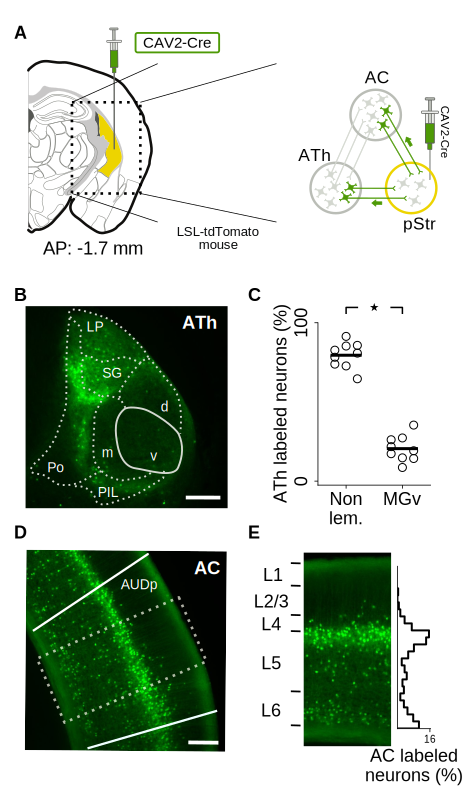
\includegraphics[height=4.1in]{figures/chapter3/fig1_anatomy}% 
  \end{center}
\caption{Neurons in auditory thalamus (ATh) and auditory cortex (AC) project to the posterior striatum (pStr).}{(A) A retrograde virus (CAV2-Cre) was injected in the posterior striatum (yellow) of LSL-tdTomato mice, shown here in a coronal brain slice.  
%
The virus is picked up by the axon terminals and transported to the cell bodies, causing excision of the loxP-flanked STOP cassette and subsequent expression of tdTomato in neurons that project to the injection location. 
%
(B) Expression of tdTomato in ATh neurons (AP -3.16 mm; v, d, and m: ventral, dorsal, and medial nuclei of the medial geniculate body, respectively. LP: lateral posterior nucleus, SG: suprageniculate nucleus, PO: posterior thalamic nucleus, PIL: posterior intralaminar thalamic nucleus).
%
Scale bar = 200 $\mu$m. 
%
(C) Most thalamic striatal-projecting neurons were located in non-lemniscal thalamic nuclei: d, m, SG, LP, PO, and PIL. 
%
Each point represents the fraction of labeled neurons for one of three interleaved sets of histological sections from each animal (3 mice, stars represent p$<$0.05). 
%
(D) Expression of tdTomato in AC neurons (AUDp: primary auditory cortex). 
%
Dotted rectangle represents cortical region shown in E. Scale bar = 200 $\mu$m. 
%
(E) Striatal-projecting neurons in AC were present across deep cortical layers with high density in the superficial portion of layer 5.
%
Results were consistent across all cortical slices analyzed. 
}
\end{figure}
%%%%%%%%%%%%%%%%%%%%%%%%%%%%%%%%%%%%%%%%%%%%%%%%%%%%%%%%%%%%%%%%%%%%%


We next sought to determine how the neurons that project to the striatum respond to sounds. 
%
We used a retrograde viral approach, similar to the technique described above, to tag striatal-projecting neurons with Channelrhodopsin-2 (ChR2).
%
This allowed us to identify these cells during extracellular recording by presenting pulses of blue light \citep{Lima2009} (\fig{\Method}).
%
A key component of this method is separating neurons that are directly activated by ChR2 from neurons that are indirectly activated by feedforward synaptic input. 
%
To achieve this, we applied two previously used criteria: reliability of responses to a train of pulses, and latency of responses to light \citep{Lima2009, Cohen2012}. 
%
To validate this approach, we blocked synaptic transmission locally in a subset of recordings by applying the AMPA glutamate receptor antagonist NBQX (\fig{\MethodDiagram}).
%
This manipulation confirmed that cells which do not respond to 5 Hz trains of light pulses (\fig{\MethodIndirectNoFollow}) or which have long latencies (\fig{\MethodLongLatency}) fail to respond to laser after NBQX, indicating that they were indirectly activated. 
%
Only neurons that were able to reliably follow a train of laser pulses with short latency had light evoked responses that persisted after synaptic transmission was blocked (\fig{\MethodDirectCellAndNBQXPop}).
%
Neurons which passed these criteria were considered directly activated by light, and therefore identified as striatal-projecting neurons (\fig{\MethodSoundCharPop}).

%%%%%%%%%%%%%%%%%%%%%%%% Figure Method %%%%%%%%%%%%%%%%%%%%%%%%%%%%%
\begin{figure}[hp]
  \begin{center}
    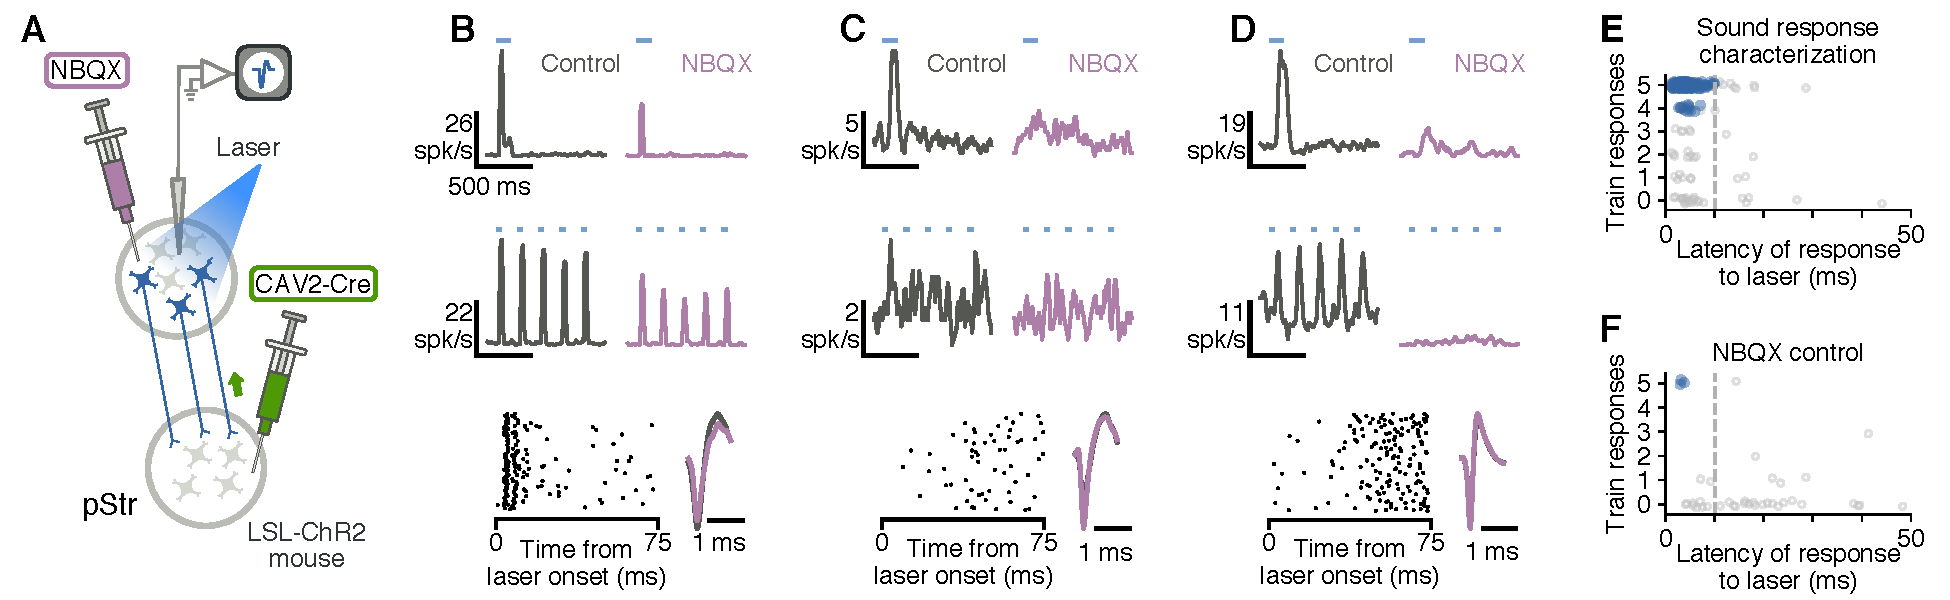
\includegraphics[width=6in]{figures/chapter3/fig2_method}% 
  \end{center}
\caption{Identification of striatal-projecting neurons during extracellular recording.}{(A) CAV2-Cre injected in the posterior striatum (pStr) of LSL-ChR2 mice travels retrogradely and causes expression of ChR2 in striatal-projecting neurons.
%
ChR2-expressing neurons were identified by their responses to laser light during extracellular recording. 
%
To validate approaches for distinguishing between ChR2-expressing neurons and neurons that respond to light due to synaptic excitation, we measured changes in light-evoked responses after blocking synaptic transmission with NBQX.
%
(B) Top row: Response of an example cortical neuron to a 100 ms pulse of blue laser light before and after application of NBQX. Middle row: This neuron responds reliably to a 5 Hz train of 10 ms laser light pulses before and after NBQX. Bottom row: This neuron responds within 10 ms of light onset (left). Spike shape was consistent before and after NBQX injection (right). 
%
(C) Example cortical neuron that responds to light (top) but cannot follow a train of laser pulses (middle). The light-evoked responses of this neuron disappear after NBQX application. 
%
(D) Example cortical neuron that responds to a train of laser pulses (middle) but has a long latency response (bottom). 
%
The light-evoked responses of this neuron disappear after NBQX application. 
%
(E) Neurons collected during sound response characterization recordings were classified as striatal-projecting if they displayed fast, reliable responses to light (blue points). Laser-responsive nerons which did not meet these criteria were excluded (grey points).
Dotted grey line represents a threshold requiring neurons to reach 1/2 of their maximum laser-evoked firing rate within 10 ms.
%
(F) Neurons collected during NBQX control experiments which continued to respond after application of NBQX display fast, reliable responses to light (blue points). Laser-responsive neurons which failed to respond after application of NBQX did not meet the criteria used to operationally define striatal-projecting neurons. 
}
\end{figure}
%%%%%%%%%%%%%%%%%%%%%%%%%%%%%%%%%%%%%%%%%%%%%%%%%%%%%%%%%%%%%%%%%%%%%


To probe the auditory responses of identified striatal-projecting neurons, we used an ensemble of stimuli including bursts of white noise, pure tones at frequencies between 2-40 kHz, and sinusoidally amplitude modulated (AM) white noise at modulation rates between 4-128 Hz. 
%
We recorded the responses of 55 tagged, sound-responsive neurons in auditory thalamus (5 mice) and 45 tagged, sound responsive neurons in auditory cortex (3 mice). 
%
As expected from the anatomical results, a large majority of neurons in auditory thalamus were recorded from non-lemniscal thalamic nuclei (85\%, 47/55, \fig{\NoiseLaserThalLocations}).
%
\fig{\NoiseLaserThalExample} shows an example thalamostriatal neuron which responds reliably to a burst of white noise.
%
\fig{\NoiseLaserACExample} shows the responses to white noise of an example auditory corticostriatal neuron.
%
Although corticostriatal neurons are present in multiple fields of the auditory cortex (\fig{\AnatomyACExample}), our experiments targeted the primary auditory cortex, such that 84\% (38/45) of recorded neurons were from the primary field (\fig{\NoiseLaserACLocations}).

These results demonstrate that both thalamus and cortex send auditory information to the striatum. We next wanted to know whether these two pathways provide redundant or complementary information about sounds to striatal neurons.

%%%%%%%%%%%%%%%%%%%%%%%% Figure Noise/Laser %%%%%%%%%%%%%%%%%%%%%%%%%%%%%
\begin{figure}[hp]
  \begin{center}
    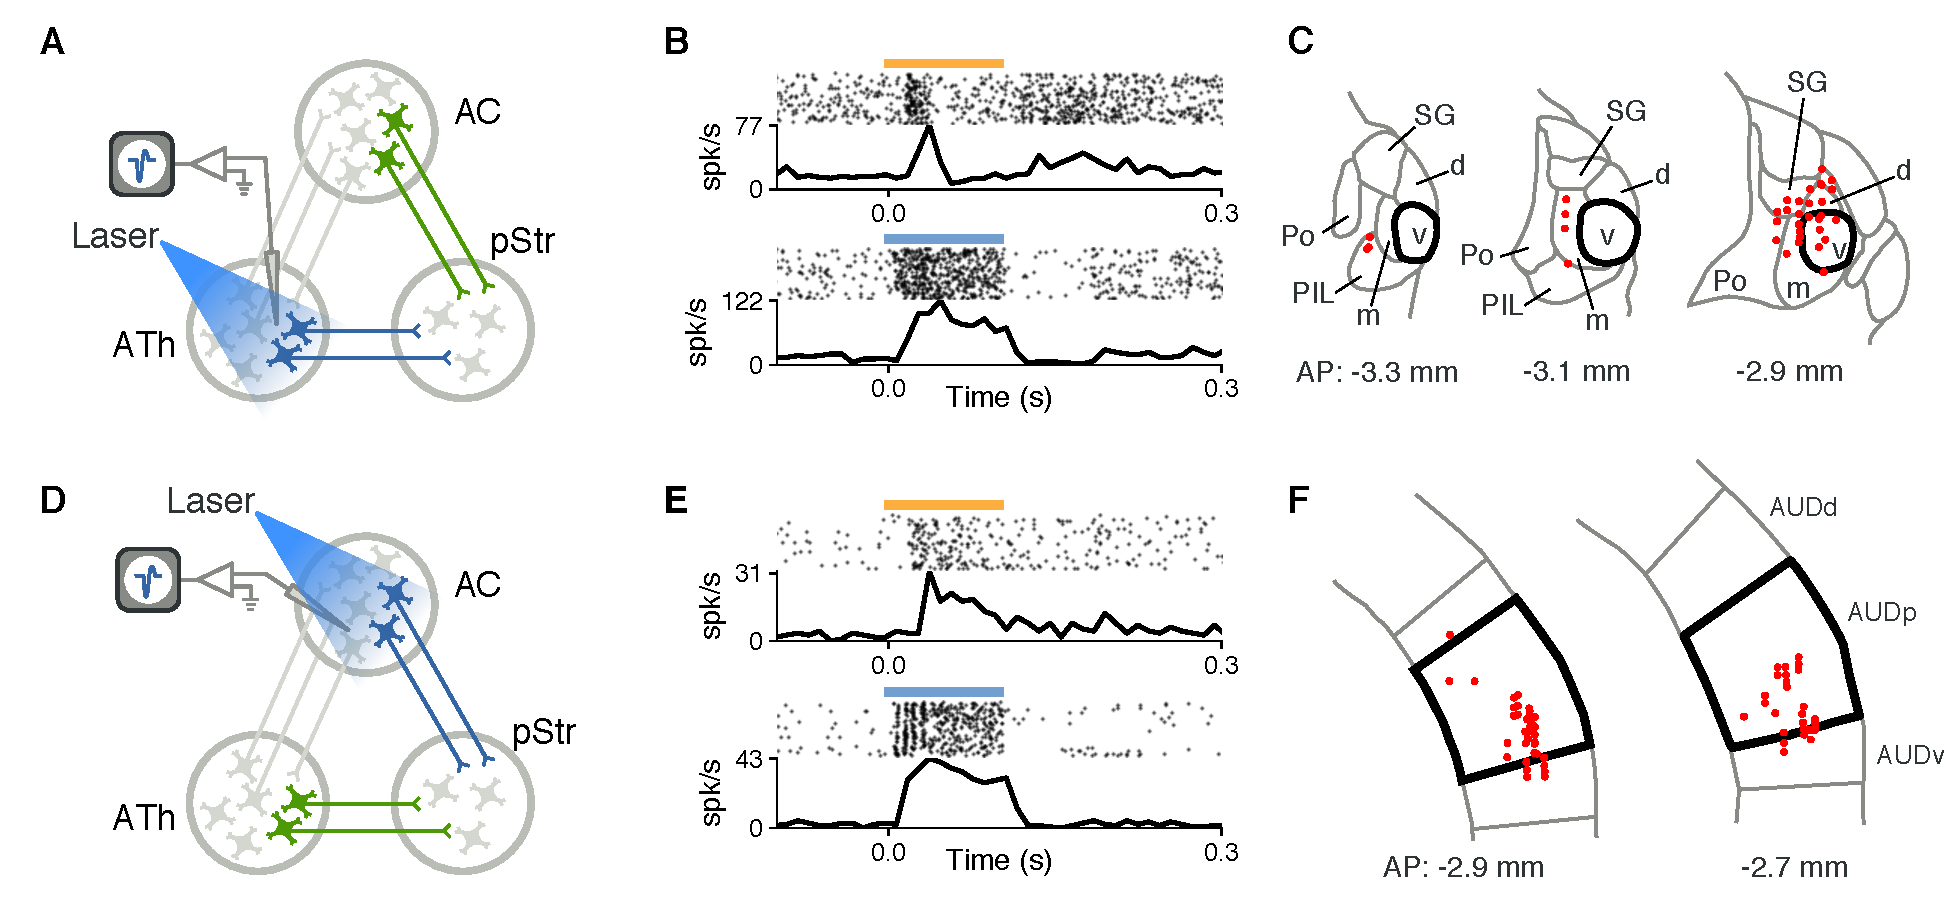
\includegraphics[width=6in]{figures/chapter3/fig3_noise_laser}% 
  \end{center}
\caption{Striatal-projecting neurons in auditory thalamus and auditory cortex display reliable sound responses. 
}{We recorded from ChR2-tagged striatal-projecting neurons in auditory thalamus (A) or auditory cortex (D).
%
(B) Example sound-evoked response and laser-evoked response from a ChR2-tagged neuron in auditory thalamus (yellow bar: 100 ms burst of 60 dB SPL white noise; blue bar: 100 ms pulse of 445 nm laser light). 
%
(C) Coronal sections showing locations of recorded tagged neurons in ATh. Each recording location was projected onto the closest example section. Thicker lines represent the border of MGv.
%
(E) Same as (B) for an example ChR2-tagged neuron in auditory cortex. 
%
(F) Coronal sections showing locations of recorded tagged neurons in auditory cortex. Each recording location was projected onto the closest example section. Thicker lines represent the border of the primary auditory field (AUDp). AUDd and AUDv are the dorsal and ventral fields, respectively. 
}
\end{figure}
%%%%%%%%%%%%%%%%%%%%%%%%%%%%%%%%%%%%%%%%%%%%%%%%%%%%%%%%%%%%%%%%%%%%%

\subsection{Thalamostriatal and corticostriatal neurons display similar sound frequency tuning bandwidth}

To determine whether thalamostriatal and corticostriatal neurons provide different information about sound frequency to the striatum, we recorded responses of identified neurons from these pathways to pure tones at frequencies between 2-40 kHz and intensities between 15-70 dB SPL. 
%
Figure 3 shows example frequency-intensity tuning curves for a ChR2-tagged neuron in auditory thalamus (\fig{\FrequencyThalExample}) and auditory cortex (\fig{\FrequencyACExample}).
%
We first analyzed the latency of the response to sound, and found that corticostriatal neurons had longer latencies than thalamostriatal neurons (p$<$0.001, Mann-Whitney U test, \fig{\FrequencyLatency}). 
%
Thalamostriatal neurons had higher baseline firing rates than corticostriatal neurons (ATh:Str median=3.75 spk/s, AC:Str median=0.82 spk/sec, p$<$0.001, Mann-Whitney U test). 
%
However, the maximum baseline-subtracted evoked firing rate was not different between thalamostriatal and corticostriatal neurons (ATh:Str median=16.32 spk/s, AC:Str median=11.81 spk/sec, p=0.18, Mann-Whitney U test). 

%%%%%%%%%%%%%%%%%%%%%%%% Figure Frequency %%%%%%%%%%%%%%%%%%%%%%%%%%%%%
\begin{figure}[hp]
  \begin{center}
    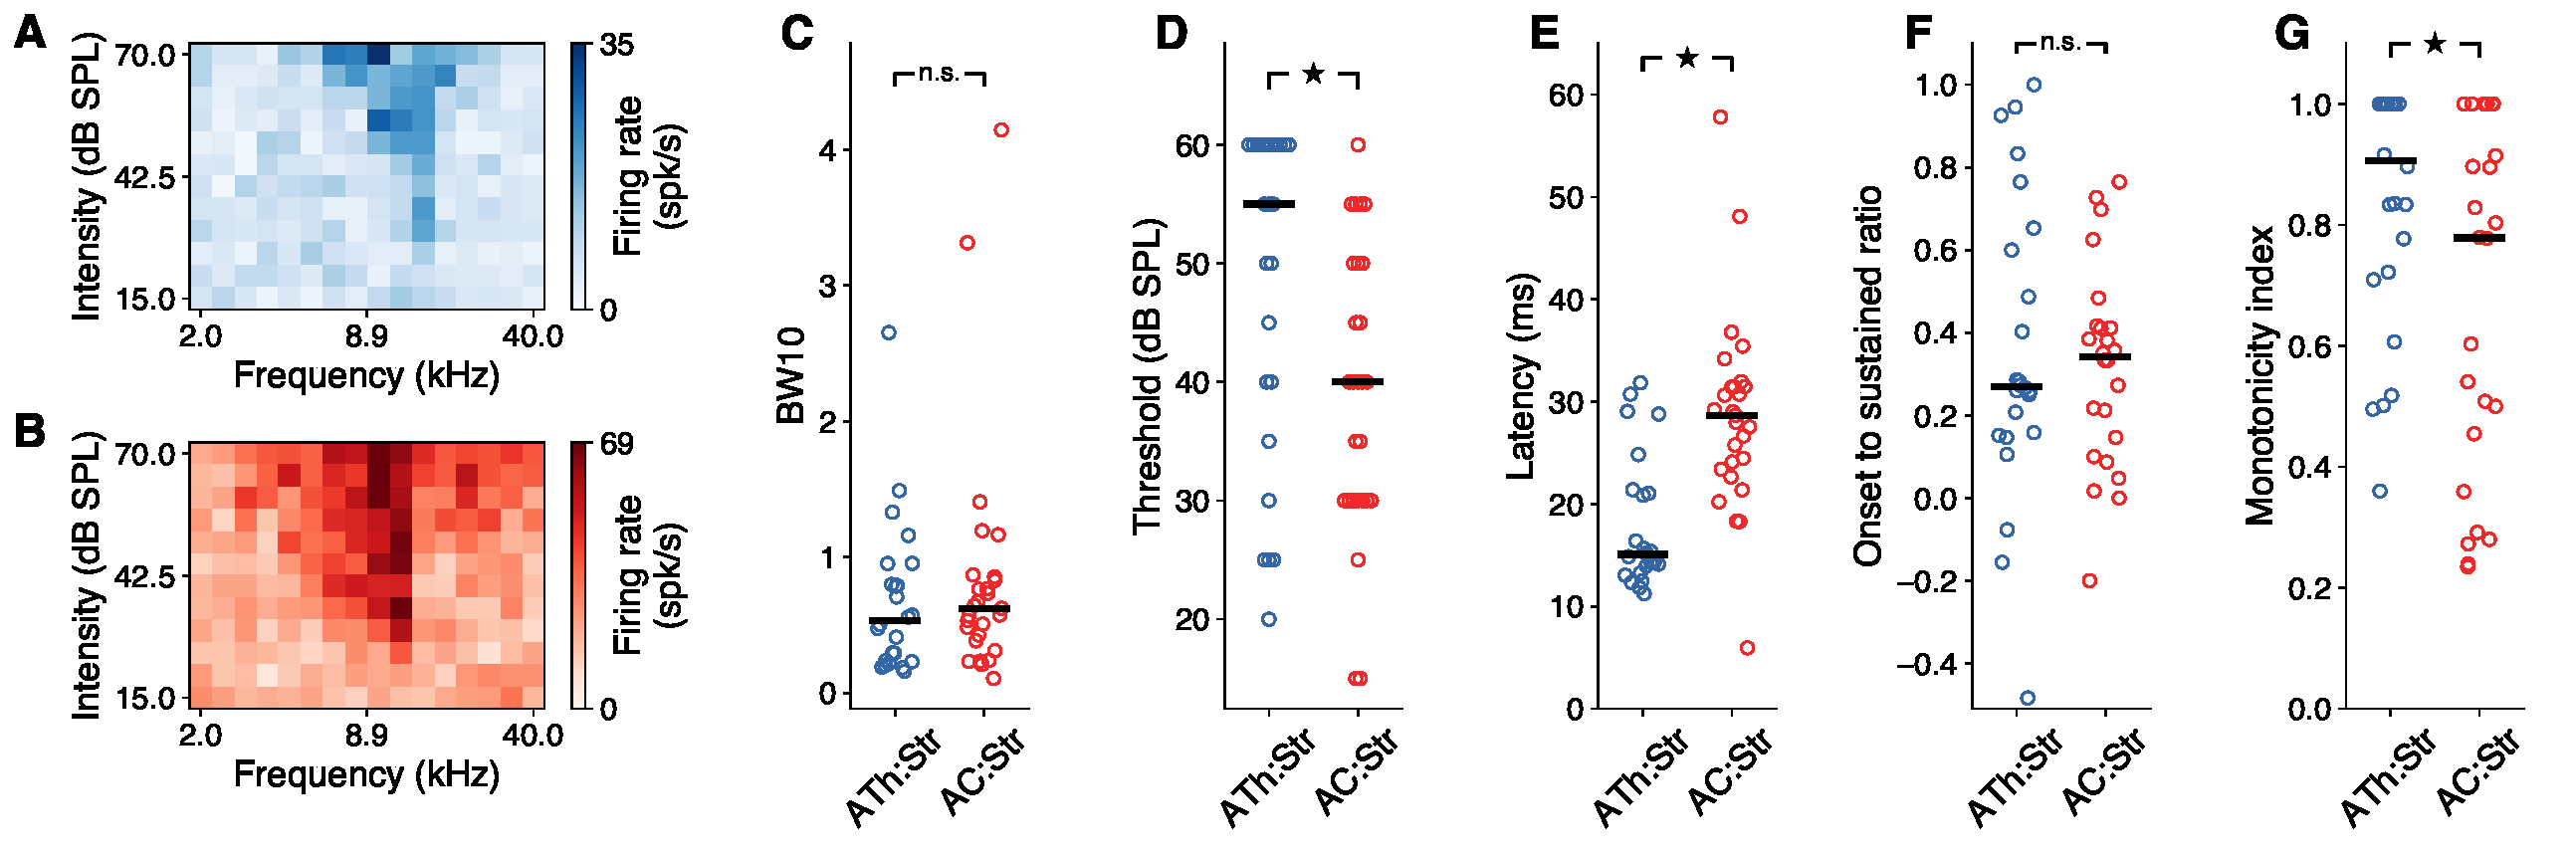
\includegraphics[width=6in]{figures/chapter3/fig4_frequency}% 
  \end{center}
\caption{Auditory thalamostriatal and corticostriatal neurons encode sound frequency with similar fidelity.}{(A) Example frequency-intensity tuning curve from a striatal-projecting neuron in auditory thalamus.
%
Tuning curves were generated by recording neural responses to 100 ms pure tone pips at 16 frequencies (2-40 kHz) and 12 intensities (15-70 dB SPL in 5 dB steps). 
%
(B) Example frequency-intensity tuning curve from a striatal-projecting neuron in auditory cortex. 
%
(C) No statistically significant difference in tuning bandwidth at 10 dB above threshold (BW10) was observed between tuned auditory thalamostriatal (n=24) and auditory corticostriatal (n=27) neurons. 
%
(D) Intensity threshold for responses to pure tones was lower in auditory corticostriatal neurons than thalamostriatal neurons. 
%
(E) Auditory thalamostriatal neurons display shorter response latencies to pure tones than corticostriatal neurons. 
%
(F) No statistically significant difference was observed in the ratio of onset spike rate to sustained spike rate between thalamostriatal and corticostriatal neurons.
%
(G) Thalamostriatal neurons display more monotonic responses to sound level than corticostriatal neurons.
%
Stars represent p$<$0.05. Black bars indicate the median value of each group.
}
\end{figure}
%%%%%%%%%%%%%%%%%%%%%%%%%%%%%%%%%%%%%%%%%%%%%%%%%%%%%%%%%%%%%%%%%%%%%

We then determined the characteristic frequency for each neuron, the threshold sound intensity required to get a response at that frequency, and the bandwidth of the tuning curve at 10 dB above that threshold (BW10). 
%
We found that corticostriatal neurons displayed lower thresholds than thalamostriatal neurons (p=0.015, Mann-Whitney U test, \fig{\FrequencyThreshold})
%
This difference could be the result of convergence from multiple lemniscal and non-lemniscal thalamic inputs onto the cortex. 
%
Calculation of BW10 was only possible for neurons that were tuned for frequency and had thresholds below 60 dB. We found 24 thalamostriatal neurons and 27 corticostriatal neurons that met these criteria.
%
Thalamostriatal and corticostriatal neurons displayed similar BW10 values (p=0.448, Mann-Whitney U test, \fig{\FrequencyBW}) suggesting that the two pathways are capable of providing frequency information to the striatum with similar fidelity. 

Additionally, we estimated how monotonic each neuron was in its response to presentations of the characteristic frequency at different intensities.
%
We found that thalamostriatal neurons displayed responses that were more monotonic with respect to sound level than corticostriatal neurons (p=0.019, Mann-Whitney U test, \fig{\FrequencyMonotonicity}). 
%
Lastly, we evaluated whether temporal response dynamics differed between thalamostriatal and corticostriatal neurons. 
%
We calculated an index that compared the strength of the onset response to sound (the first 50 ms of a neuron's response) with the sustained component of the response (from 50 ms to 100 ms after the beginning of the response). 
%
We found no difference in this index between thalamostriatal and corticostriatal neurons (p=0.845, Mann-Whitney U test, \fig{\FrequencyOnsetivity}). 


Because our method for retrograde ChR2-tagging is not guaranteed to label every striatal-projecting neuron, a subset of untagged neurons may still project to the striatum. Despite this caveat, we evaluated whether there were any differences between tagged neurons and neighboring untagged neurons. We observed no differences in frequency tuning metrics between these populations in either thalamus (BW10: p=0.54, threshold: p=0.28, latency: p=0.39) or cortex (BW10: p=0.79, threshold: p=0.95, latency: p=0.17).

Overall, while thalamostriatal and corticostriatal pathways display different latencies, and corticostriatal neurons are more likely to display non-monotonic tuning for sound level, comparison of BW10 values suggests that both pathways are capable of conveying information about sound frequency to the striatum with similar fidelity. 
%
We next sought to determine how these two pathways encode temporal features of sound.

\subsection{Thalamostriatal and corticostriatal neurons convey different information about temporal features of sounds}

To determine whether thalamus and cortex provide different information about temporal features to the striatum, we analyzed the responses of striatal-projecting neurons to amplitude modulated (AM) noise stimuli at modulation rates from 4 Hz to 128 Hz.
%
We found 36 tagged neurons in auditory thalamus and 24 neurons in auditory cortex with reliable responses to AM noise stimuli.
%
Neurons along the auditory pathway can respond to AM noise by synchronizing their spiking output to the period of the modulation, or by firing during the stimulus presentation without regard to the modulation period.
%
In addition, neurons that synchronize their firing to low AM rates may not do so for high AM rates.
%
Figure 4 shows example responses to AM sounds in two striatal-projecting neurons in auditory thalamus (\fig{\AMThalExamples}) and auditory cortex (\fig{\AMACExamples}).
%
Thalamostriatal neurons synchronized to many of the AM rates presented, but their average firing rate over the duration of the stimulus often depended little on the AM rate.
%
In contrast, corticostriatal neurons appeared less synchronized to the period of the AM stimulus, especially at fast AM rates, and their evoked average firing rate often varied as a function of the AM rate.
%
We found that the ratio of onset to sustained firing rates in response to AM sounds was similar between thalamostriatal and corticostriatal neurons (p=0.23, Mann-Whitney U test).

%%%%%%%%%%%%%%%%%%%%%%%% Figure AM %%%%%%%%%%%%%%%%%%%%%%%%%%%%%
\begin{figure}[hp]
  \begin{center}
    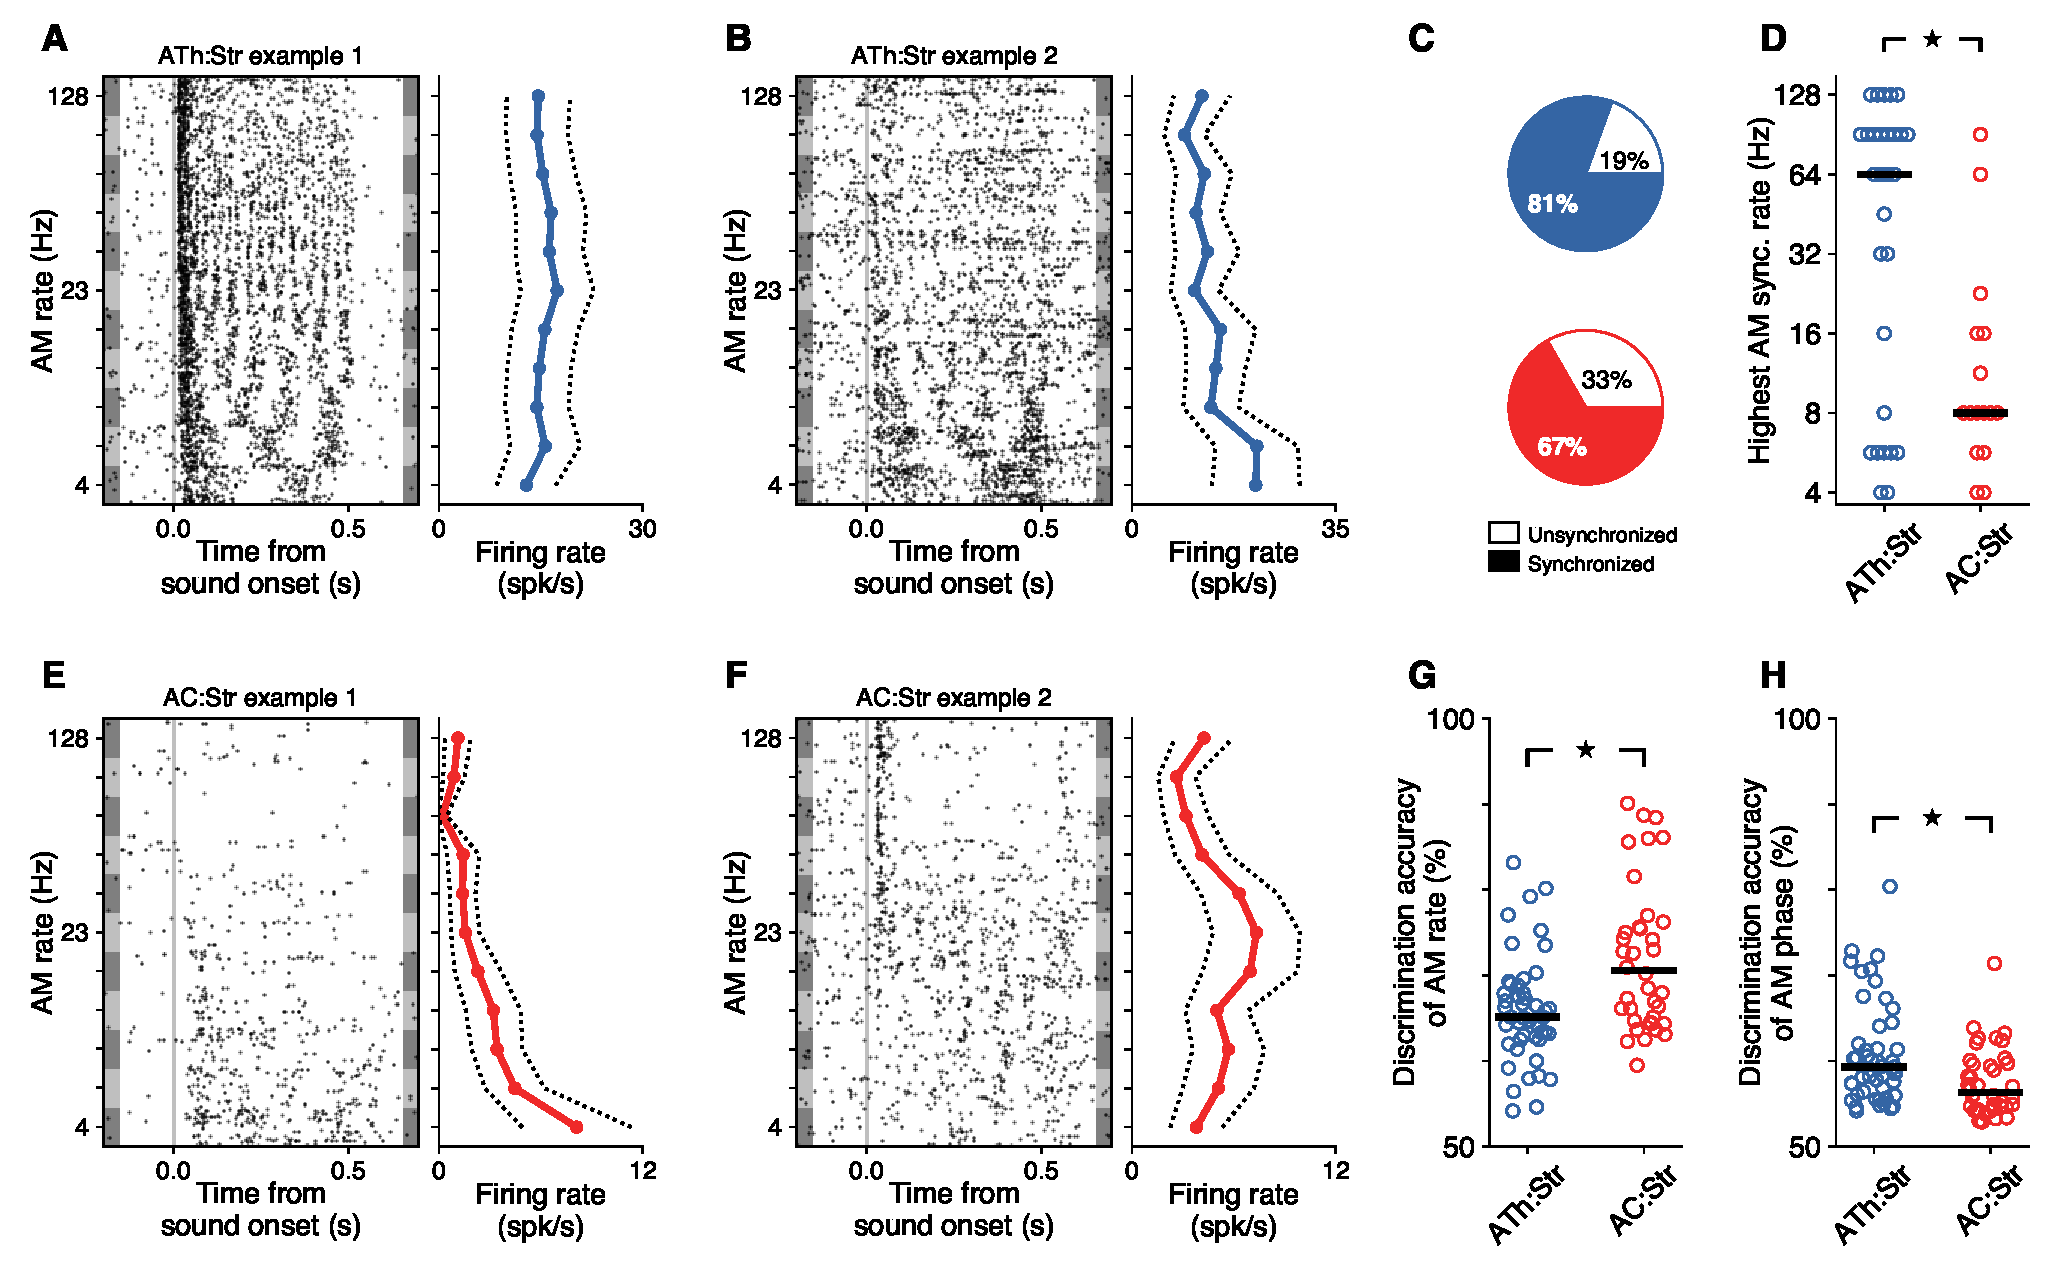
\includegraphics[width=6in]{figures/chapter3/fig5_am}% 
  \end{center}
\caption{Thalamostriatal and corticostriatal neurons convey different information about temporal features of sounds.}{(A, B) Example responses of two auditory thalamostriatal neurons to amplitude modulated (AM) white noise at different modulation rates. 
%
Average firing rates vary little as a function of AM rate. 
%
Dotted lines indicate 1 s.d.
%
AM stimuli consisted of 500 ms bursts of white noise at 60 dB SPL, modulated by a sinusoid (4-128 Hz).
%
Modulation depth was 100\%. 
%
(C) Both thalamostriatal (7/36=19\%) and corticostriatal (8/24=33\%) populations contained some neurons unable to synchronize to any AM stimulus presented. 
%
Filled areas represent neurons able to synchronize to at least one AM stimulus.
%
(D) Thalamostriatal neurons display higher maximum synchronization rates compared to corticostriatal neurons.
%
(E, F) Example responses of two auditory corticostriatal neurons to AM noise at different modulation rates. 
%
Average firing rates are modulated by AM rate. 
%
Dotted lines indicate 1 s.d.
%
(G) A linear discriminator is better able to tell apart preferred from least-preferred AM rate using average stimulus-evoked firing rates of corticostriatal neurons than thalamostriatal neurons. 
%
(H) A linear discriminator is better able to tell apart preferred from least-preferred AM phase using firing rates from thalamostriatal neurons than from corticostriatal neurons. Discrimination accuracy was calculated separately for each AM rate. Each dot represents the average accuracy across all AM rates for each neuron.
%
Stars indicate p$<$0.05. Black bars indicate the median value of each group. 
}
\end{figure}
%%%%%%%%%%%%%%%%%%%%%%%%%%%%%%%%%%%%%%%%%%%%%%%%%%%%%%%%%%%%%%%%%%%%%

To quantify the difference in encoding of AM stimuli between thalamostriatal and corticostriatal neurons, we first determined the highest AM rate to which each neuron was able to synchronize its firing.
%
We found that thalamostriatal neurons were able to synchronize their firing to higher AM rates than corticostriatal neurons (p$<$0.001, Mann-Whitney U test, \fig{\AMSync}).
%
There was also a non-significant trend towards cortical neurons being more likely to show unsynchronized responses to all AM rates we tested: 33\% (8/24) of auditory cortical neurons \emph{vs.}\ 19\% (7/36) of thalamic neurons (p=0.24, Fisher’s exact test, \fig{\AMPies}).
%
These results suggest that auditory thalamostriatal and corticostriatal neurons represent AM sounds in different ways.

To further address these differences in neural representations, we estimated how accurately a downstream linear classifier could discriminate between each neuron's preferred and least-\\preferred AM rate, given average firing rates for each trial.
%
We found that discrimination accuracy was better for corticostriatal neurons than for thalamostriatal neurons (ATh:Str mean=65.9\%, AC:Str mean=72\%, p=0.001, Mann-Whitney U test, \fig{\AMRateDiscrim}).
%
We also calculated discrimination accuracy using spikes only from the sustained portion of the response, and found that this did not affect accuracy in either thalamostriatal or corticostriatal neurons (ATh:Str mean=66\%, ATh:Str with- \emph{vs.} without-onset p=0.68, Mann-Whitney U test. AC:Str mean=70.9\%, AC:Str with- \emph{vs.} without-onset p=0.57, Mann-Whitney U test.)

In addition, to evaluate the amount of information that neurons provide about the full range of AM rates beyond the preferred and least-preferred stimuli, we calculated the mutual information between the response on each trial and the AM rate.
%
We found that corticostriatal neurons provided more information about AM rate than thalamostriatal neurons  (p=0.012, Mann-Whitney U test).
%
Corticostriatal neurons on average provided 0.06 bits of information per trial, with some cells providing up to 0.23 bits. 
%
Thalamostriatal neurons provided an average of 0.03 bits and a maximum of 0.16 bits.
%

We next tested how well a downstream classifier could discriminate between preferred and least-preferred phase of the stimulus envelope.
%
To do this, we aligned each neuron's spikes to the phase of the AM stimulus presented on each trial, and calculated the firing rate during each phase quadrant. 
%
We found that discrimination accuracy for phase was better for thalamostriatal neurons than for corticostriatal neurons (p$<$0.001, \fig{\AMPhaseDiscrim}).
%
We did not observe any differences in AM response metrics between tagged and untagged neurons either in thalamus (highest sync rate: p=0.57, rate discrimination accuracy: p=0.31, phase discrimination accuracy: p=0.75) or cortex (highest sync rate: p=0.27, rate discrimination accuracy: p=0.26, phase discrimination accuracy: p=0.11).

These results suggest that thalamus and cortex provide complementary information about amplitude modulated sounds to the striatum.
%
The average firing rates of neurons in the corticostriatal pathway provide an explicit representation of the modulation rate of a stimulus, while thalamostriatal neurons provide information about the precise timing of acoustic events. 

% TODO: Be consistent about Discussion / Conclusion across chapters
\section{Discussion}

By recording sound-evoked responses of striatal-projecting neurons from auditory thalamus and auditory cortex of awake mice, we found that these two pathways send complementary information about the features of sounds.
%
While thalamic and cortical neurons send largely redundant information to the striatum about sound frequency, thalamostriatal neurons provide signals with shorter latency. 
%
Corticostriatal neurons, meanwhile, are more sensitive to pure tones at low intensities and are more likely to display non-monotonic responses to sound level (\emph{i.e.}, intensity tuning).

Moreover, corticostriatal neurons more accurately represent the amplitude modulation rate in their average firing rate, while the responses of thalamostriatal neurons more closely follow rapid variations in stimulus amplitude.
%
Our results suggest that these two pathways could be differentially recruited during sound-driven behaviors depending on the requirements of the task.

\subsection{Auditory cortical projections to the striatum}
Our anatomical results suggest that neuronal projections from auditory cortex to the posterior striatum in the mouse arise mostly from cortical layer 5, with some projections from layer 6. 
%
These results are consistent with a recent anatomical study in the rat using CAV2 as a retrograde tracer \citep{Jiang2018}, although the projection to striatum from layer 6 was not observed in an earlier study in the rat using a different intersectional viral approach \citep{Znamenskiy2013}. 
%
One challenge with retrograde tracing methods is the possibility of the virus being picked up by damaged fibers of passage. However, it is unlikely that this possibility explains the robust expression seen in cortical layer 6 since our experiments show little expression in MGv, a nucleus which sends neuronal projections to primary auditory cortex that also course through the posterior striatum.

Multiple cortical regions, in addition to the auditory cortex, target the posterior portion of the dorsal striatum \citep{Hunnicutt2016}.
%
Consistent with these anatomical patterns, we observed labeled neurons in cortical regions outside of auditory cortex, including regions of somatosensory cortex overlying the injection site in the posterior striatum.
%
The presence of labeled neurons outside the desired auditory cortical region raises the possibility that the virus spread beyond the target striatal area (\emph{e.g.}, by leakage along the injection tract). However, because expression was restricted to the same laminar distribution observed in auditory cortex, the possibility of major leakage does not seem likely, as this would result in less organized patterns of expression of the fluorophore.

\subsection{Representation of sound features across the auditory pathway}
%
Previous studies in anesthetized animals comparing neurons in auditory cortex and lemniscal auditory thalamus have found little difference in frequency tuning bandwidth between these regions \citep{Miller2002}. 
%
Within the thalamus, frequency tuning bandwidth differs between the dorsal (MGd) and ventral (MGv) nuclei of the medial geniculate body, while other nuclei (MGm and POL) show overlapping tuning with MGv \citep{Anderson2011}.
%
Consistent with previous studies \citep{Doron1999}, our anatomical results indicate that the thalamostriatal projection largely originates from neurons across non-lemniscal nuclei. 
%
These observations imply that, without the ability to record directly from striatal-projecting neurons, it would be challenging to predict what frequency information is conveyed by these neurons. 
%

Our results indicate that, although some thalamostriatal neurons are located in MGd, frequency tuning bandwidth between thalamostriatal and corticostriatal neurons is largely overlapping. 
%
Despite the similarity in tuning bandwidth we observe between thalamostriatal and corticostriatal neurons, it is possible that the relative effects of cortical and thalamic pathways on striatal responses are additionally shaped by the strength of the synapses in these pathways and by the patterns of convergence onto striatal neurons to produce appropriate behavioral outputs. 
%
For instance, differences in release probability and short term plasticity have been shown between thalamostriatal and corticostriatal synapses \citep{Ding2008}, and these two pathways target different compartments of striatal cells \citep{Smith2004}. 
%
Notably, with the parameters used in this study, we were not able to calculate BW10 for many thalamostriatal neurons (56\%, compared to 40\% of AC:Str neurons) because either CF was not captured, or we had no data for 10 dB above threshold. This suggests that tuning may be more common among corticostriatal neurons across the range of intensities tested.
 
The responses to amplitude modulated (AM) sounds that we observed across cortex and thalamus are consistent with previous work showing that responses to these sounds change from being synchronized with the stimulus at the auditory periphery to being largely unsynchronized in higher auditory cortical areas (reviewed in \cite{Joris2004} and \cite{Wang2008}). 
%
For example, in primates, neurons in A1 have mixed temporal (synchronized) and rate-coded (unsynchronized) representations, while responses of most neurons in secondary auditory fields do not synchronize to the period of the modulation \citep{Bendor2007, Niwa2013}.

In the auditory thalamus, the representation of AM stimuli differs across nuclei. 
%
MGm and SG display largely synchronized responses, MGd displays responses that are largely unsynchronized, and MGv displays a mixture of the two response types \citep{Bartlett2013}. 
%
Given these results, the thalamostriatal pathway could contain a mixture of different AM response types. 
%
Our experiments, using a method to interrogate neurons specifically from this pathway, suggest that synchronized responses predominate among thalamic neurons that project to the striatum.

In neural circuits responsible for discriminating AM rate, having inputs where the overall spike count is highly correlated with AM rate (as seen in corticostriatal neurons) means a simple threshold can accomplish the discrimination task. 
%
In contrast, inputs in which firing is synchronized with the variations in amplitude, but that do not change the overall spike-count for the duration of the stimulus (as is common in thalamostriatal neurons), would require additional processing for implementing AM rate discrimination.
%
As representations of AM sounds are transformed from synchronized to rate-coded across the auditory pathway, these signals become progressively more useful to an area performing AM rate discrimination.

\subsection{Subcortical outputs of the auditory thalamus}
%
The posterior striatum is not the only subcortical region where auditory thalamic and cortical signals converge.
%
The lateral amygdala, the most extensively studied subcortical output of the auditory thalamus, also receives extensive inputs from auditory cortex \citep{Ledoux2000}.
%
%
The thalamoamygdala pathway is capable of exhibiting learning-induced changes in synaptic strength thought to underlie amygdala-dependent aversive conditioning \citep{McKernan1997}.
% 
Lesions to the entire auditory thalamus disrupt fear conditioning to sounds, but lesions to either the corticoamygdala or the thalamoamygdala pathway alone leave fear conditioning intact \citep{Ledoux1983, Romanski1992}.
% 
Thus, the thalamoamygdala and the corticoamygdala pathways are both independently able to facilitate fear conditioning. 
%
Similarly, auditory discrimination tasks involving simple, narrowband stimuli require posterior striatal circuits \citep{Guo2018} but can be performed after extensive lesions of auditory cortex \citep{Gimenez2015}, suggesting that auditory corticostriatal and thalamostriatal pathways are independently able to mediate this discrimination. 

Our results suggest that thalamic neurons that project to the striatum are located in many of the same nuclei as neurons that project to the lateral amygdala \citep{Doron1999}. 
%
Although neurons in the amygdala encode both negative and positive valence of sensory cues \citep{Tye2008}, these neurons seem to play only a minimal role in associations between stimuli and actions to obtain reward \citep{Baxter2002}. 
%
Regions of the dorsal striatum, in contrast, have been shown to play a key role in reward-related motor learning \citep{Wickens2003, Balleine2007}.
% 
These differences suggest that the thalamostriatal and thalamoamygdala pathways play complementary roles in sound-driven behavior. 

%
Thalamic projections to subcortical forebrain structures are predominant in phylogenetically primitive vertebrates with less developed neocortices \citep{Ebner1969, Kudo1986}, and it is likely that the last common ancestor between mammals and other vertebrates displayed similar neural pathways. 
%
This suggests the possibility that the outputs from the auditory thalamus to the striatum and amygdala in mammals are vestigial, an evolutionary holdover. 
%
However, we find that the thalamostriatal and corticostriatal pathways send complementary information about sound features to the striatum. 
%
Therefore, by using information arriving from the thalamus, rather than signals from cortex alone, striatal circuits might help achieve better performance in certain kinds of auditory tasks.

\subsection{Striatum-mediated learning with sensory inputs from two parallel pathways}

Recent studies have proposed a model of reward-related sound discrimination learning in which the synapses between auditory cortical neurons that represent a stimulus feature and neurons in the striatum that can drive appropriate actions are potentiated \citep{Xiong2015}. 
%
While it is not known whether thalamostriatal synapses undergo the same type of stimulus-specific plasticity, thalamic signals (potentially via the striatum) seem sufficient to mediate associations between narrowband sounds and rewarded actions \citep{Gimenez2015, Guo2018}.
%

Depending on the demands of a task, striatal neurons may selectively potentiate distinct input sensory pathways.
%
For tasks requiring discrimination between AM rates, the cortical inputs provide signals that can be decoded with a linear classifier without further processing.
%
In contrast, for tasks requiring precise timing, striatal neurons could potentiate thalamic inputs and take advantage of the features provided by this pathway. 
